\part{Atomic actions}
\section{Learning goals}
\begin{itemize}
\item  A thorough understanding of the problems Atomic Actions are meant to solve and how these motivates the different aspects of Atomic Actions.
\item Ability to use and implement Atomic Actions, including the mechanisms providing the start, side and end boundaries.
\item Understanding the motivation for using Asynchronous Notification in Atomic Actions.
\item A coarse knowledge of how the mechanisms for Asynchronous Notification in C/Posix, ADA and Java works.
\end{itemize}

\section{What are atomic actions}
\subsection{Motivation for using atomic actions}
An Atomic Action is a design framework for damage confinement and error recovery. Before we go into the actual details, lets just give a heads up and say that a transaction discussed in the last part is in fact an atomic action structure with backward error recovery. We know from before that should have \textit{recovery line} to avoid domino effect if we have backward error recovery. The question is how we achieve synchronization of recovery points. With atomic actions, we get the structure necessary to achieve both backward and forward error recovery. The recovery synchronization is not a straight line here, it is a registration of when a task enters an atomic action and if something goes wrong within it, all tasks in it are rolled back to the state they were in when they entered the atomic action. The general usage of atomic cations is for when several groups of concurrent tasks need to be structured to allow for coordination of their activities. The \textbf{atomic action} is required for each group of tasks to execute their joint activity. It should be mentioned that a single task may also want to protect itself from interference from other tasks. Atomic actions can therefore be said to involve one or more tasks and be a method for structuring these tasks such that they can operate on different parts of a single task concurrently. Figure \ref{fig: atomic_actions} shows a simplistic representation of how atomic actions work.

\begin{figure}[H]
\centering
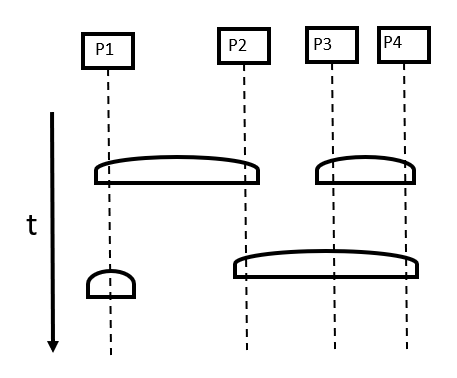
\includegraphics[width=0.6\textwidth]{figures/Fault_Tolerance/atomic_actions.PNG}
\label{fig: atomic_actions}
\caption{Illustration of how atomic actions can work}
\end{figure}

\subsection{Different ways to define atomic actions }
\begin{enumerate}
\item An action is atomic if the tasks performing it are not aware of the existence of any other active tasks, and no other active tasks is aware of the activity of the tasks during the time the tasks are performing the action. 
\item An action is atomic if the tasks performing it do not communicate with other tasks while the action is being performed.
\item An atomic action has tasks that cannot detect state change except those performed by themselves and they do not reveal their state changes until the action is complete.
\item Atomic actions are by other tasks considered to be indivisible and instantaneous such that the effects on the system are as if they were interleaved as opposed to concurrent.  
\end{enumerate}

\subsection{Requirements for atomic actions}
\begin{itemize}
\item \textbf{Well-defined boundaries} - Each atomic action should have a \textit{start}, an \textit{end} and a \textit{side boundary}. Start boundary is the location in each task involved in the atomic action where the action is deemed to start. The end boundary is where it is deemed to end and the side boundary separates tasks involved with the atomic action from those not involved.
\item \textbf{Indivisibility (isolation)} - an atomic action must not allow the exchange of any information between the tasks on each side of the side boundary. If two atomic actions share data trough a Resource Manager then the value is determined by strict sequencing. There is no implied \textit{synchronization} at the start of an atomic action, but tasks are not allowed to leave the atomic action until all tasks are willing and able to leave.
\item \textbf{Nesting} - Atomic actions may be nested as long as they do not overlap with other atomic actions. In general only \textit{strict nesting} allowed where one is completely contained within the other.
\item \textbf{Concurrency} - It should be possible to execute different atomic actions concurrently
\end{itemize}

\subsection{Standard Atomic Actions implementation}
Transaction mentioned in last part is a good example of an atomic action.
Start boundary:
\begin{enumerate}
\item Dynamic (call to e.g. \textit{startTransactionWithWork()}
\end{enumerate}
Side boundary:
\begin{enumerate}
\item Locking, no unlocking before safe state (end boundary).
\end{enumerate}
End boundary:
\begin{enumerate}
\item Vote counting (two-phase commit)
\item Synchronization primitive barrier that no one can pas through before everyone has arrived.
\end{enumerate}

\section{Language-specific atomic action implementation}
\todo{Fill out more here}
Java:
\begin{itemize}
\item Synchronized methods, wait, notify / notifyAll
\item Asynchronous exceptions
\end{itemize}
Ada:
\begin{itemize}
\item Protected objects
\item Function procedures and entries with guards.
\end{itemize}
C/POSIX
\begin{itemize}
\item pthread cancel
\item setjmp and longjmp
\end{itemize}

\section{Asynchronous notification}
Asynchronous notification is a bit like interrupts in hardware. It is a way to distribute error information instead of using the commit structure discussed or some polling regime to make forward error recovery possible instead of just backward error recovery. To get a recoverable action we must be able to get the attention of a task involved in the action that an error has occurred in another task involved in the action. This is achieved with an asynchronous notification mechanism which most programming languages and operating systems support. As with exceptions, there are two basic models; \textbf{resumption} and \textbf{termination}. 

\subsection{Resumption (event handling)}
Behaves like a software interrupt. A task indicates which events it is willing to handle; when the event is signaled the task is interrupted and an event handler is executed. Afterwards the task resumes from where it was when the interrupt came in.

\subsection{Termination model}
Each task specifies a domain of execution during which it is prepared to receive  an asynchronous notification that will cause the domain to be terminated. In less formal wording, this means that after we handle the error we terminate what we were doing and start somewhere else in the code, for example lower down.

\subsection{The user need for asynchronous notification}
Fundamental need is to enable tasks to respond \textit{quickly} to a condition which has been detected by another task. There are several occasions where polling for events or waiting for the event to occur is inadequate:
\begin{itemize}
\item \textbf{Error recovery} - When groups of tasks undertake \textit{atomic actions}, an error detected in one task requires all other tasks to participate in the recovery as the work they are now doing might be useless if the error has propagated. The form of asynchronous notification we will use here for termination is \textit{Asynchronous Transfer of Control (ATC)}
\end{itemize}

\subsection{Language specific asynchronous notification implementation}
\subsubsection{C/POSIX}
Supports the resumption model. Has a set of predefined signals and 3 ways in which a process can deal with a signal. 
\begin{enumerate}
\item \textbf{Block} - Handle it later or accept it
\item \textbf{Handle} - Setting a function to be called whenever it occurs
\item \textbf{Ignore} - The signal is simply lost
\end{enumerate}
If we want asynchronous transfer of control we can use \textbf{setjmp} and \textbf{longjmp} mechanisms. 
\begin{verbatim}
#include <stdio.h>
#include <setjmp.h>

static jmp_buf buf;

void second(void) {
    printf("second\n");			 	   // prints
    longjmp(buf,1); 				// jumps back to where setjmp was called
}

void first(void) {
    second();
    printf("first\n"); 					// does not print
}

int main() {
    if ( ! setjmp(buf) ) {
        first(); 								 // when executed, setjmp returns 0
    } else { 									// when longjmp jumps back, setjmp returns 1
        printf("main\n"); // prints
    }
    return 0;
}
\end{verbatim}
When program above executed it will return "second main"

\subsubsection{Asynchronous notification in Ada}
The asynchronous notification facilities in Ada allow an application to respond to among other things asynchronous transfer of control (ATC) requests on a task - supporting a termination model. There is no generalized model for resumption in Ada. To emphasize that ATC is a form of communication and synchronization, the mechanism  is built on top of the inter-task communication facility.

We will look at of \textit{Asynchronous select} here. 
\newpage
\begin{lstlisting}
select
    Trigger.Event;
    -- optional sequence of statements to be 
    -- executed after the event has been received
then abort
    -- abortable sequence of statements
end select;
\end{lstlisting}
It is best explained with an example
\begin{lstlisting}
task Server is
	entry ATC_EVENT;
end Server;

task To_Be-Interrupted;

task body Server is
begin
	...
    accept ATC_EVENT do 
    	Seq2; 
    end ATC_EVENT;
    ...
end Server;

task body To_Be_Interrupted is
begin
	...
    select -- ATC statement
    	Server.ATC_EVENT;
        Seq3;
    then abort
    	Seq1; 
        -- the work here is the normal operation work
        -- Will be interrupted if it times out or event happens
    end select;
    Seq4;
    -- Seq4 comes after the asynchronous select, it cannot be interrupted.
    ...
end To_Be_Interrupted;
\end{lstlisting}
When the above ATC statement is executed, the statements which are executed will depend on the order of events that occur. See page 257 in BW chapter 7. The Ada ATC facility described above is used to implement both forward and backward error recovery.

\newpage

\subsubsection{Asynchronous notification in Java}
ATC here also. Focus on Real-Time Java.
\begin{itemize}
\item Built on Java exceptions
\item Can be blocked
\end{itemize}




